\begin{adjustwidth*}{}{-2.25in}
\textbf{{\large Exercises}}
\setlength{\columnsep}{25pt}
\begin{multicols*}{2}
\noindent Terms and Concepts \small
\begin{enumerate}[1)]
\item T/F: The chain rule describes how to evaluate the derivative of a composition of functions.
\item T/F: The Generalized Power Rule states that $\ds \frac{d}{dx}\Big( g(x)^n\Big) = n\big(g(x)\big)^{n-1}$.
\item T/F: $\ds \frac{d}{dx}\big(3^x\big) \approx 1.1\cdot3^x$.
\item T/F: $\ds \frac{dx}{dy} = \frac{dx}{dt}\cdot \frac{dt}{dy}$
\item Let $u(x)$ be a differentiable function.  For each of the following functions, determine the derivative.  Each response will involve $u$ and/or $u'$.
\ba
	\item $p(x) = e^{u(x)}$
	\item $q(x) = u(e^x)$
	\item $r(x) = \cot(u(x))$
	\item $s(x) = u(\cot(x))$
	\item $a(x) = u(x^4)$
	\item $b(x) = u^4(x)$
\ea
\end{enumerate} 

\noindent {\normalsize Problems} \small

\noindent {\bf In exercises 6--23, compute the derivative of the given function.}

\begin{enumerate}[1),resume]
\item $\ds f(x) = (4x^3 - x)^{10}$
\item $\ds f(t) = (3t-2)^5$
\item $\ds g(x) = (\sin(x) + \cos(x))^3$
\item $\ds h(t) = e^{3t^2 + t -1}$
\item $\ds f(x) = \left( x + \frac{1}{x} \right)^4$
\item $\ds f(x) = \cos(3x)$
\item $\ds g(x) = \tan(5x)$
\item $\ds h(t) = \sin^4(2t)$
\item $\ds p(t) = \cos^3(t^2 + 3t + 1)$
\item $\ds h(r) = 4^r$
\item $\ds g(t) = 5^{\cos(t)}$
\item $\ds v(t) = 15^2$
\item $\ds m(w) = \frac{3^w}{2^w}$
\item $\ds m(w) = \frac{3^w + 1}{2^w}$
\item $\ds f(x) = \frac{3^{x^2} + x}{2^{x^2}}$
\item $\ds f(x) = x^2 \sin(5x)$
\item $\ds g(t) = \cos(t^2 + 3t) \sin(5t - 7)$
\item $\ds g(x) = \cos\left( \frac{1}{x} \right) e^{5x^2}$
\end{enumerate}

\noindent {\bf In exercises 24--27, find the equation of the tangent line to the graph of the function at the given point.}

\begin{enumerate}[1),resume]
\item $\ds f(x) = (4x^3 - x)^{10}$ at $x = 0$
\item $\ds f(t) = (3t-2)^5$ at $t = 1$
\item $\ds g(x) = (\sin(x) + \cos(x))^3$ at $x = \pi/2$
\item $\ds h(t) = e^{3t^2 + t -1}$ at $t = -1$

\item Consider the basic functions $f(x) = x^3$ and $g(x) = \sin(x)$.
\ba
	\item Let $h(x) = f(g(x))$.  Find the exact instantaneous rate of change of $h$ at the point where $x = \frac{\pi}{4}.$
	\item Which function is changing most rapidly at $x = 0.25$:  $h(x) = f(g(x))$ or $r(x) = g(f(x))$?  Why?
	\item Let $h(x) = f(g(x))$ and $r(x) = g(f(x))$.  Which of these functions has a derivative that is periodic?  Why?
\ea

\item If a spherical tank of radius 4 feet has $h$ feet of water present in the tank, then the volume of water in the tank is given by the formula
$$V = \frac{\pi}{3} h^2(12-h).$$
\ba
	\item At what instantaneous rate is the volume of water in the tank changing with respect to the \emph{height} of the water at the instant $h = 1$?  What are the units on this quantity?
	\item Now suppose that the height of water in the tank is being regulated by an inflow and outflow (e.g., a faucet and a drain) so that the height of the water at time $t$ is given by the rule $h(t) = \sin(\pi t) + 1$, where $t$ is measured in hours (and $h$ is still measured in feet).  At what rate is the height of the water changing with respect to time at the instant $t = 2$?
	\item Continuing under the assumptions in (b), at what instantaneous rate is the volume of water in the tank changing with respect to \emph{time} at the instant $t = 2$?  
	\item What are the main differences between the rates found in (a) and (c)?  Include a discussion of the relevant units.
\ea
\end{enumerate}

%------------------------------------------
% END OF EXERCISES ON FIRST PAGE
%------------------------------------------
\end{multicols*}
\end{adjustwidth*}

\clearpage

\begin{adjustwidth*}{}{-2.25in}
\setlength{\columnsep}{25pt}
\begin{multicols*}{2}\small

\begin{enumerate}[1),start=30]
\item Let functions $p$ and $q$ be the piecewise linear functions given by their respective graphs below.  Use the graphs to answer the following questions.
\begin{center}
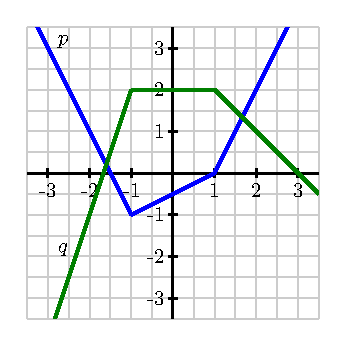
\includegraphics{figures/2_1_Ez3.eps}
\end{center}
\ba
	\item Let $C(x) = p(q(x))$.  Determine $C'(0)$ and $C'(3)$.
	\item Find a value of $x$ for which $C'(x)$ does not exist.  Explain your thinking.
	\item Let $Y(x) = q(q(x))$ and $Z(x) = q(p(x))$.  Determine $Y'(-2)$ and $Z'(0)$.	
\ea
\end{enumerate}

%---------------------------------------------
% END OF EXERCISES ON SECOND PAGE
%---------------------------------------------
\end{multicols*}
\end{adjustwidth*}

\afterexercises